\ifx\wholebook\relax \else

\documentclass[b5paper]{ctexart}
\usepackage[nomarginpar
  %, margin=.5in
]{geometry}

\addtolength{\oddsidemargin}{-0.05in}
\addtolength{\evensidemargin}{-0.05in}
\addtolength{\textwidth}{0.1in}

\usepackage[cn]{../prelude}

\setcounter{page}{1}

\begin{document}

\title{复数}

\author{刘新宇
\thanks{{\bfseries 刘新宇} \newline
  Email: liuxinyu99@hotmail.com \newline}
  }

\maketitle
\fi

\markboth{复数}{数的旅程}

\ifx\wholebook\relax
\chapter{复数}
\fi

%% On earth there is nothing great but man; and in man there is nothing great but mind.
\epigraph{地球上最伟大的是人,人之中最伟大的是心灵}{威廉·汉密尔顿}

读过金庸武侠小说的读者一定对“华山论剑”津津乐道。天下武林中的顶级高手约定在华山比武论剑。大家各自有秘不外传的绝世武功,并通过比武确定谁是真正的天下武功第一。十六世纪的意大利也上演了精彩的华山论剑。只不过这是一场没有刀光剑影、没有拳脚身法,而是关于数学与荣誉的挑战。1535年2月13日深夜,在威尼斯的家中,塔尔塔利亚

\begin{figure}[htbp]
  \centering
  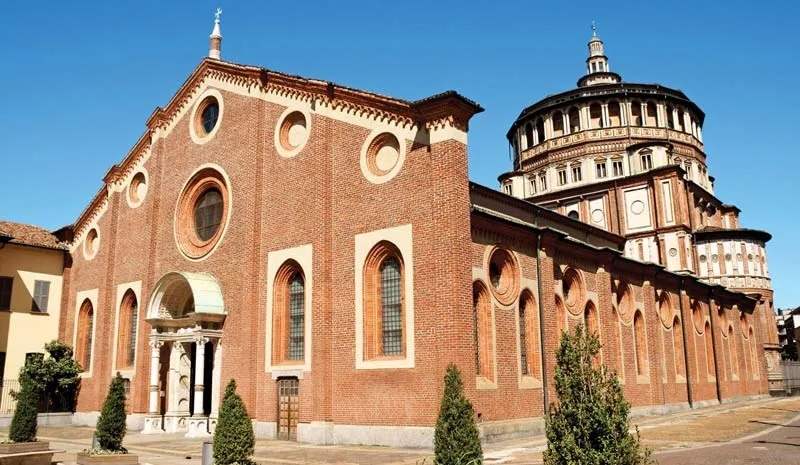
\includegraphics[scale=0.33]{img/churchmilan}
  \caption{米兰圣母玛丽亚感恩大教堂}
 \label{fig:church-Milan}
\end{figure}

%% del Ferro:德尔・费罗(意大利数学家尼科洛・德尔・费罗,Niccolò del Ferro,15 世纪末至 16 世纪初,首次解出一元三次方程的一类特殊情况)
%% Fior:费奥尔(意大利数学家安东尼奥・马里亚・费奥尔,Antonio Maria Fior,16 世纪,曾与塔尔塔利亚就三次方程解法展开竞赛)
%% Ferrari:费拉里(意大利数学家洛多维科・费拉里,Lodovico Ferrari,16 世纪,在卡尔达诺指导下首次解出一元四次方程)

\section{三次方程}
解三次方程的历史

\section{佚名数学家}
\subsection{复数的几何意义和运算法则}
\subsection{匿名作者阿尔冈}
\subsection{代数基本定理}

\section{e的传奇}
\subsection{e的诞生}
\subsection{最美公式}

\section{新世界的大门}
\subsection{小试牛刀}
麦钦公式、正五边形作图
\subsection{费马大定理与高斯整数}
\subsection{抽象的数}
理想数
\subsection{新数的构造-代数数}

\ifx\wholebook\relax \else
\section{参考答案}
\shipoutAnswer

\begin{thebibliography}{99}
\subimport{inc/}{bib-zh-cn}
\end{thebibliography}

\expandafter\enddocument
\fi
